%%%%%%%%%%%%%%%%%%%%%%% file template.tex %%%%%%%%%%%%%%%%%%%%%%%%%
%
% This is a general template file for the LaTeX package SVJour3
% for Springer journals.          Springer Heidelberg 2010/09/16
%
% Copy it to a new file with a new name and use it as the basis
% for your article. Delete % signs as needed.
%
% This template includes a few options for different layouts and
% content for various journals. Please consult a previous issue of
% your journal as needed.
%
%%%%%%%%%%%%%%%%%%%%%%%%%%%%%%%%%%%%%%%%%%%%%%%%%%%%%%%%%%%%%%%%%%%
%
% First comes an example EPS file -- just ignore it and
% proceed on the \documentclass line
% your LaTeX will extract the file if required
\begin{filecontents*}{example.eps}
%!PS-Adobe-3.0 EPSF-3.0
%%BoundingBox: 19 19 221 221
%%CreationDate: Mon Sep 29 1997
%%Creator: programmed by hand (JK)
%%EndComments
gsave
newpath
  20 20 moveto
  20 220 lineto
  220 220 lineto
  220 20 lineto
closepath
2 setlinewidth
gsave
  .4 setgray fill
grestore
stroke
grestore
\end{filecontents*}
%
\RequirePackage{fix-cm}
%
%\documentclass{svjour3}                     % onecolumn (standard format)
%\documentclass[smallcondensed]{svjour3}     % onecolumn (ditto)
\documentclass[smallextended]{svjour3}       % onecolumn (second format)
%\documentclass[twocolumn]{svjour3}          % twocolumn
%
\smartqed  % flush right qed marks, e.g. at end of proof
%
\usepackage{graphicx}
%
\usepackage{hyperref}
%
\usepackage{mathptmx}      % use Times fonts if available on your TeX system
%
\usepackage{comment}
% insert here the call for the packages your document requires
\usepackage{latexsym}
% etc.
%
% please place your own definitions here and don't use \def but
\newcommand{\hospital}{`\textit{San Carlo di Nancy}' hospital }
%
% Insert the name of "your journal" with
%\journalname{BISE}
%
\makeatletter
\newcommand{\setword}[2]{%
  \phantomsection
  #1\def\@currentlabel{\unexpanded{#1}}\label{#2}%
}
\makeatother
\begin{document}

\title{Applying process mining techniques in a real healthcare case study%\thanks{Grants or other notes
%about the article that should go on the front page should be
%placed here. General acknowledgments should be placed at the end of the article.}
}
%\subtitle{Do you have a subtitle?\\ If so, write it here}

%\titlerunning{Short form of title}        % if too long for running head

\author{M. Mecella \and
		F. Covino \and 
		A. Marrella\and \\
		S. Agostinelli}

%\authorrunning{Short form of author list} % if too long for running head

\institute{M. Mecella \at
			  Professor in Engineering in Computer Science at Sapienza University of Rome\\
              %Tel: +39 0677274028 \\
			  %Fax: +39 0677274002 \\
              \email{mecella@dis.uniroma1.it}           %  \\
%             \emph{Present address:} of F. Author  %  if needed
           \and
           A. Marrella \at
              Postdoctoral research fellow in Computer Science and Engineering at Sapienza University of Rome\\
              %Tel: +39-06-77274012 \\
			  %Tel: +39-06-77274013 \\
			  %Fax: +39-06-77274002 \\
              \email{marrella@dis.uniroma1.it}           %  \\
%             \emph{Present address:} of F. Author  %  if needed
           \and
           F. Covino \at
           CMMI Business Analyst at ENAV\\
           \email{federico.covino@gmail.com}
           \and
           S. Agostinelli \at
           Graduated in Computer Engineering at Sapienza University of Rome\\
           \email{simone.agostinelli.sa@gmail.com}
}

\date{Received: date / Accepted: date}
% The correct dates will be entered by the editor


\maketitle

\begin{abstract}
%Insert your abstract here. Include keywords, PACS and mathematical
%subject classification numbers as needed.
The healthcare organizations are under increasing pressure to improve productivity, gain competitive advantage and reduce costs. For this reason, healthcare organizations, such as hospitals try to streamline their processes. In this paper we demonstrate the applicability of process mining in the healthcare domain, using a real case study of \hospital in Rome (GVM Group). We apply process mining techniques to obtain meaningful knowledge about the patient careflows from so-called event logs, obtained from raw data of hospital information systems. We analyzed these logs using the ProM framework from three different perspectives: the control flow perspective, the organizational perspective and the timing perspective. The results show that process mining can be used to provide new insights that facilitate the improvement of existing careflows.
\keywords{Process mining \and Healthcare \and ProM}
% \PACS{PACS code1 \and PACS code2 \and more}
% \subclass{MSC code1 \and MSC code2 \and more}
\end{abstract}
\clearpage
\section{Introduction}
Nowdays, the hospitals try to streamline their processes in order to deliver high quality care while at the same time improving revenues and reducing costs. More and more pressure is put on hospitals to work in the most efficient way as possible, whereas in the future, an increase in the demand for care is expected. A complicating factor is that healthcare is characterized by highly complex and extremely flexible patient care processes, also referred to as `\textit{careflows}'. In healthcare organisations, a wide range of processes with different characteristics and requirements are daily managed and executed. The delivery of complex care may involve several departments and organisations, and requires an active collaboration between different professionals and practitioners having heterogeneus skills. Healthcare is thus widely recognised as one of the most promising, yet challenging, domains for the adoption of process-oriented solutions. We demonstrates the applicability of process mining in the healthcare domain, using a real case study of \hospital in Rome (GVM Group). We apply process mining techniques to obtain meaningful knowledge about the patient careflows from so-called `\textit{event logs}' obtained from raw data of hospital information systems. Process mining aims at extracting process knowledge from that logs in order to discover, for example, both typical paths followed by particular groups of patients and strong collaboration between different hospitalization wards. We analyzed the different careflows both under the control flow perspective (emphasizing the differences between the process models obtained from different cluster of patients), the organizational perspective (looking at the social networks we were able to discover the relationship between the resources of the patient careflows) and the performance perspective (looking at the timing perspective of different activities performed by the patients we were able to discover bottlenecks in the patient careflows). In order to do so, we extracted the event logs from the raw datasets of \hospital and we analyzed them using \textit{ProM}: the process mining framework. The datasets in question are the following:
\begin{itemize}
\item \textit{Ambulatori} (outpatient clinic): each row stores the information about a single healthcare service.
\item \textit{Pronto soccorso} (emergency room): each row represents a single emergency room activity.
\item \textit{Ricoveri} (hospitalizations): each row represents a single hospitalization taken by a patient.
\end{itemize}
These three datasets contain raw data about patients treated in both year 2016 and May 2017 for which all the treatment activities have been recorded. We did not use any a-priori knowledge about the careflows of the patients of \hospital and did not have any process model at hand. The data analyzed are the standard ones of the National Health Service (Servizio Sanitario Nazionale) that the hospitals interchanged with the Regional Authorities (Enti Regione). Therefore the presented analysis can be replicated nationwide.%This paper is structured as follows: Section provides a detailed explanation of the tools used within ProM in order to derive process models, social networks and transition systems from relevant event logs. In Section we will emphasize the results obtained by applying process mining techniques. Section concludes the case study.
\clearpage

%\label{adtool}
%Your text comes here. Separate text sections with
%\section{Section title}
%\label{sec:1}
%Text with citations \cite{RefB} and \cite{RefJ}.
%\subsection{Subsection title}
%\label{sec:2}
%as required. Don't forget to give each section
%and subsection a unique label (see Sect.~\ref{sec:1}).
%\paragraph{Paragraph headings} Use paragraph headings as needed.
%\begin{equation}
%a^2+b^2=c^2
%\end{equation}
\section{Analysis} \label{analysis}
In this section, we discuss the results obtained by applying process mining techniques (process discovery, social network analysis and performance analysis) on the datasets of \hospital already `\textit{converted}' to event logs: `\textit{Ambulatori}', `\textit{Pronto soccorso}' and `\textit{Ricoveri}'. The process mining techniques we used for discovering the process model of the totality of patients (blueprint) are: the \textit{Alpha Miner} algorithm, the \textit{Heuristic Miner} algorithm and the \textit{Inductive Miner} algorithm. In order to establish which process model out of three is representing better the behaviour observed in the event log, and therefore which mining algorithm is the best, we computed the four quality metrics replay fitness, precision, generalization and simplicity. ProM 6.7 allows to compute replay fitness, precision and generalization only. Therefore simplicity is calculated on the basis of this metric: \#$activities \;+\;$\#$splits \;+\; $\#$joins$. The grater is the value, the less is the simplicity of the process model. At the end, the best algorithm will be chosen on the basis of the just mentioned quality metrics. Since the inductive visual miner is high parametrisable (i.e., we can set a-priori the replay fitness we would like to reach in order to obtain a process model in function of this fitness value) therefore it's the algorithm with the best compromise between the just mentioned quality metrics. For this reason, we picked the inductive visual miner as process discovery technique. After discovered the blueprint of all the three datasets, we have performed ad-hoc analysis for these set of clusters:
\begin{itemize}
\item foreign patients [\setword{1}{Word:foreign}] vs. italian patients [\setword{2}{Word:italian}]
\item patients with an age lower or equal than 25 years (resident in Latium)[\setword{3}{Word:young}] vs. patients with an age greater than 25 years (resident in Latium) [\setword{4}{Word:old}]
\end{itemize}
Only for `\textit{Ricoveri}' dataset we have performed a further in depth analysis for these specialist branches: \textit{chirurgia generale}, \textit{medicina generale} and \textit{ortopedia and traumatologia} looking at both pre-operative hospitalization time (the time a patient is waiting for the surgical intervention) and post-operative hospitalization time (the time a patient is waiting for being discharged).
\clearpage
\subsection{Ambulatori dataset} \label{analysis:1}
The \setword{blueprint}{Word:bpprocmod} in terms of process model is the following:
\begin{figure}[htbp]
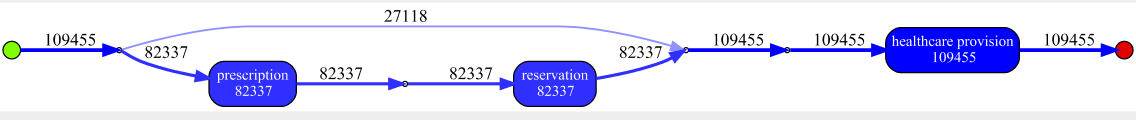
\includegraphics[width=\textwidth , keepaspectratio]{AmbulatoriInductiveVisualMiner.png}
\caption{Clinical path (Totality of patients)}
\end{figure}\\
Looking at the figure, we can see that the most of the patients takes the medical prescription and asks for a reservation before the healthcare provision. From the organizational point of view, the \setword{social network}{Word:ambsocnet} derived is as follows:
\begin{figure}[htbp]
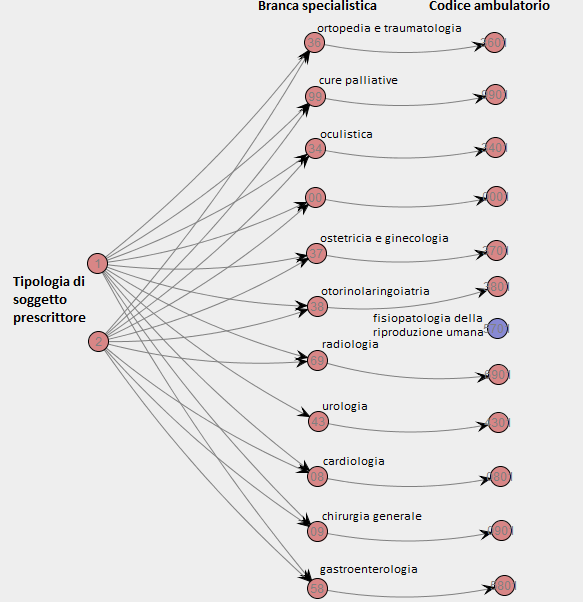
\includegraphics[width=0.75\textwidth, keepaspectratio]{AmbulatoriSocialNetwork}
\caption{Social network (Totality of patients)}
\end{figure}\\
From the picture points out that the types of prescriptive subjects involved in prescriptions are both `\textit{1}' (medico di medicina generale) and `\textit{2}' (medico specialista dipendente da struttura pubblica). They are connected with the specialist branches accredited for the healthcare provision, since the prescriptive subject chooses the specialist branch when he compiles the medical prescription. Notice that the outpatient clinic `\textit{5701}' (Fisiopatologia della riproduzione umana) is not involved in any social relation, because all the patients go in that outpatient clinic without prescription. Indeed the process model followed by these patients is composed by only one activity, the `\textit{healthcare provision}' activity:
\begin{figure} [htbp]
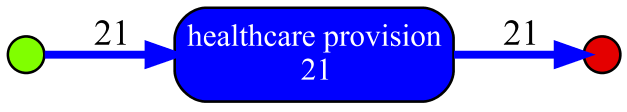
\includegraphics[width = 0.5\textwidth, keepaspectratio]{AmbulatoriInductiveVisualMiner5701}
\caption{Fisiopatologia della riproduzione umana}
\end{figure}\\
On the other hand, regarding the performance perspective we have obtained:
\begin{figure} [htbp]
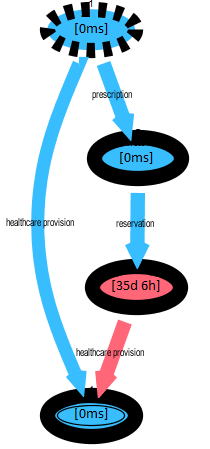
\includegraphics[width=0.3\textwidth, keepaspectratio]{AmbulatoriTransitionSystemSojourn}
\caption{Transition System (Totality of patients)}
\end{figure}\\
We can see that the most of time, %(35 days 6 hours in avg)
from the sojourn time point of view, is spent on the activity `\textit{reservation}' where the patient is waiting for the healthcare provision. The standard deviation is very high, meaning that the patients are spread out over a wide range of time, therefore the mean is not significant at all. Then, we have repeated the same analysis for different cluster of patients. We started with both the clusters [\ref{Word:foreign}] and [\ref{Word:italian}] obtaining the following process models:
\begin{figure} [htbp]
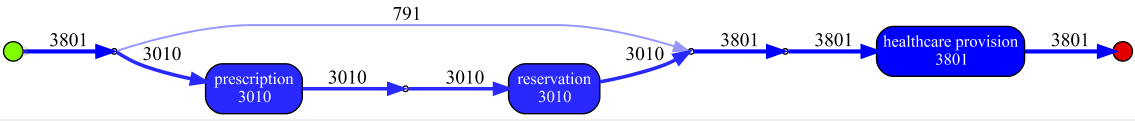
\includegraphics[width=\textwidth , keepaspectratio]{AmbulatoriInductiveVisualMinerForeigns}
\caption{Clinical path (Foreign patients)}
\end{figure}\\
\begin{figure} [htbp]
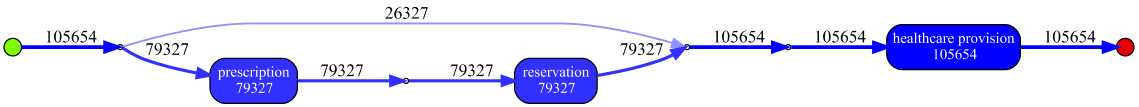
\includegraphics[width=\textwidth , keepaspectratio]{AmbulatoriInductiveVisualMinerItalians}
\caption{Clinical path (Italian patients)}
\end{figure}\\
Both the process models are identical to the \ref{Word:bpprocmod}, the only difference is on the number of process executions (3801 for [\ref{Word:foreign}] and 105654 for [\ref{Word:italian}]). Furthermore, looking at both the figures, we can see that the most of both foreign and italian patients take the medical prescription and ask for a reservation before the healthcare provision. From the organizational point of view, the social networks derived from both the clusters [\ref{Word:foreign}] and [\ref{Word:italian}] are as follows:

\begin{figure} [htbp]
\begin{minipage}[t]{0.5\textwidth}
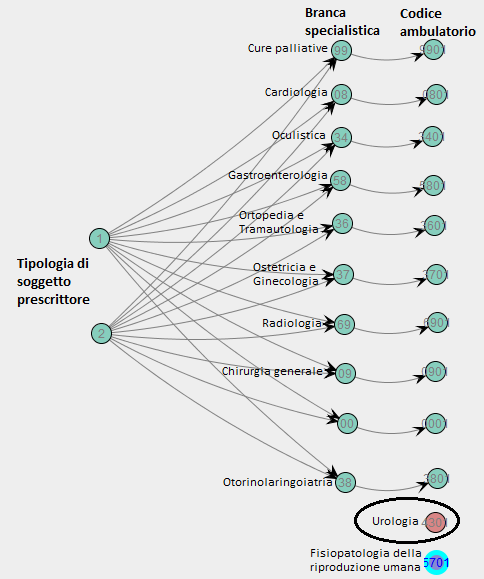
\includegraphics[width=0.75\textwidth, keepaspectratio]{AmbulatoriSocialNetworkForeigns}
\caption{Social Network (Foreign patients)}
\end{minipage}
\begin{minipage}[t]{0.5\textwidth}
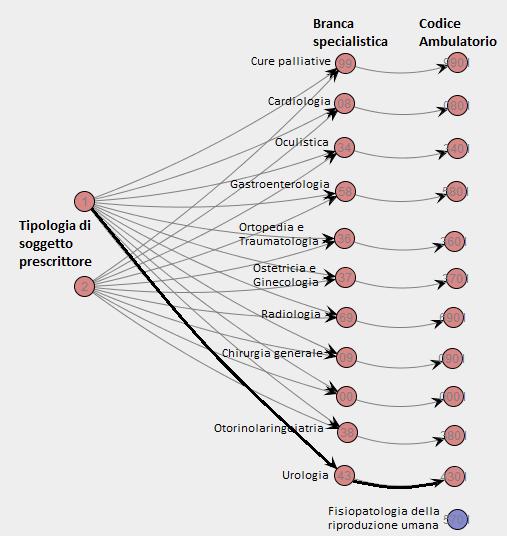
\includegraphics[width=0.83\textwidth, keepaspectratio]{AmbulatoriSocialNetworkItalians}
\caption{Social Network (Italian patients)}
\end{minipage}
\end{figure}
\noindent
Looking at the pictures, the social networks of the patients belonging from both the clusters [\ref{Word:foreign}] and [\ref{Word:italian}] involve the same resources as the blueprint \ref{Word:ambsocnet}. The only difference is on the outpatient clinic `\textit{4301}' (Urologia): the foreign patients go in this outpatient clinic without medical prescription instead the italian patients with a medical prescription compiled only from `\textit{1}' (medico di medicina generale) .This means all the foreign patients going in `\textit{4301}' perform only one activity, the `\textit{healthcare provision}'activity:
\begin{figure} [htbp]
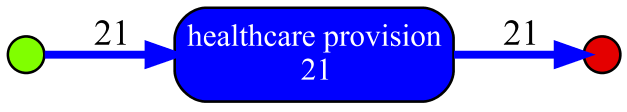
\includegraphics[width=0.5\textwidth, keepaspectratio]{AmbulatoriInductiveVisualMinerForeigns4301}
\caption{Urologia (Foreign patients)}
\end{figure}
\clearpage
\noindent
Looking at the performance perspective, in particular at the \textit{sojourn time} point of view, we obtained:
\begin{figure} [htbp]
\begin{minipage}[t]{0.5\textwidth}
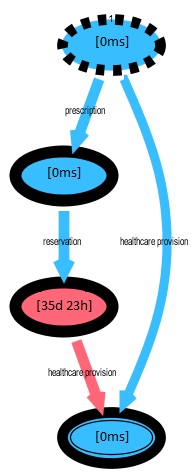
\includegraphics[width=0.5\textwidth, keepaspectratio]{AmbulatorioSojournForeigns}
\caption{Transition system (Foreign patients)}
\end{minipage}
\begin{minipage}[t]{0.5\textwidth}
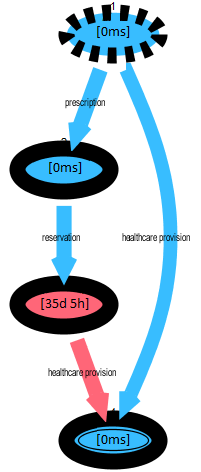
\includegraphics[width=0.5\textwidth, keepaspectratio]{AmbulatorioSojournItalians}
\caption{Transition system (Italian patients)}
\end{minipage}
\end{figure}\\
At first glance, looking at the two transition systems we can see that the states associated with activities belonging to the cluster [\ref{Word:italian}] have a border ticker than the states associated with activities belonging to the cluster [\ref{Word:foreign}], since the cluster of foreign patients contains a number of
patient's cases strictly lower than the cluster of italian patients. The same argument applies to arcs. Moreover, we can see that the most of time, for both the clusters [\ref{Word:foreign}] and [\ref{Word:italian}], is spent on the activity `\textit{reservation}' where a patient is waiting for the healthcare provision. %the average sojourn time for this activity is 35 days 23 hours for foreign patients and 35 days 25 hours for italian patients.
The avg sojourn time of both the clusters is equal (more or less) to the one of the blueprint.\\
Now we can consider another set of clusters: patients belonging both to [\ref{Word:young}] and [\ref{Word:old}]. The derived process models are the following:
\begin{figure} [htbp]
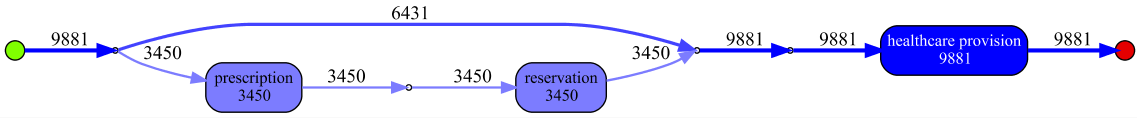
\includegraphics[width=\textwidth]{AmbulatoriInductiveVisualMinerYoungs}
\caption{Clinical path ($\leq$25 years)}
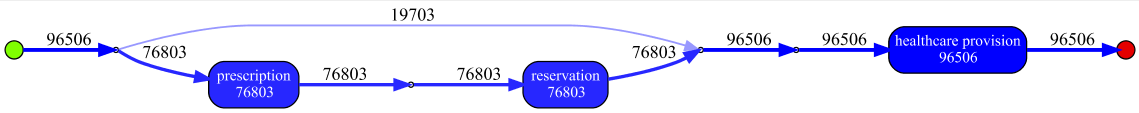
\includegraphics[width=\textwidth]{AmbulatoriInductiveVisualMinerOlds}
\caption{Clinical path ($>$25 years)}
\end{figure}\\
Both the process models are identical to the \ref{Word:bpprocmod}, but there are an interesting difference regarding the behaviour of the patients belonging to both the clusters [\ref{Word:young}] and [\ref{Word:old}], in particular regarding the most frequent path. The most frequent path taken by the patients with an age lower than 25 years (resident in Latium) is the one made up by the `\textit{healthcare provision}' activity (they go directly in outpatient clinic), instead, the most frequent path taken by the patients with an age grater or equal than 25 years (resident in Latium) is made up by the following activities: `\textit{prescription}' $ \rightarrow $ `\textit{reservation}' $ \rightarrow$ `\textit{healthcare provision}' (they take the medical prescription, then they ask for a reservation for perfoming the healthcare provision). Another difference which points out is on the number of process executions (9881 for [\ref{Word:young}] and 96506 for [\ref{Word:old}]).\\
From the organizational point of view, the social networks derived from both the clusters [\ref{Word:young}] and [\ref{Word:old}] are as follows:
\begin{figure} [htbp]
\begin{minipage}[t]{0.5\textwidth}
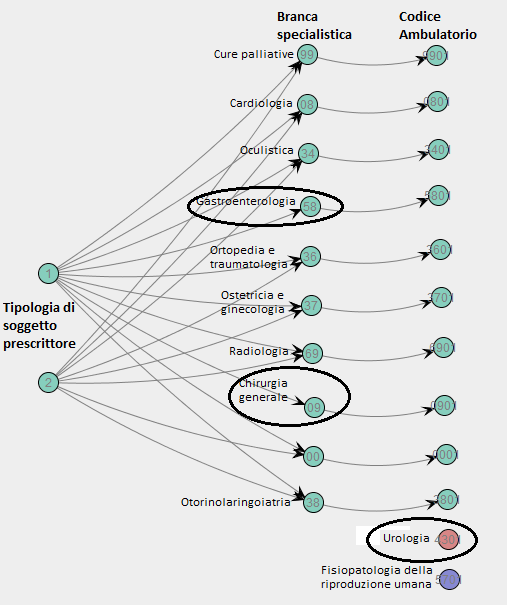
\includegraphics[width=0.89\textwidth]{AmbulatoriSocialNetworkYoungs}
\caption{Social network ($\leq$25 years)}
\end{minipage}
\begin{minipage}[t]{0.5\textwidth}
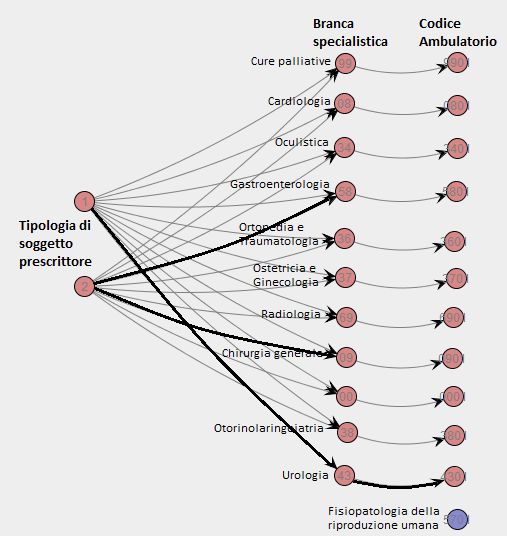
\includegraphics[width=\textwidth]{AmbulatoriSocialNetworkOlds}
\caption{Social network ($>$25 years)}
\end{minipage}
\end{figure}\\
Looking at the pictures, the social networks of the patients belonging from both the clusters [\ref{Word:young}] and [\ref{Word:old}] involve the same resources as the blueprint \ref{Word:ambsocnet}. The main difference is on the outpatient clinic `\textit{4301}' (Urologia): the patients with an age lower than 25 years (resident in Latium) go in this outpatient clinic without medical prescription, instead, the patients with an age greater or equal than 25 years (resident in Latium) go in this outpatient clinic with a medical prescription compiled only by `\textit{1}' (medico di medicina generale). This means all the patients belonging to the cluster [\ref{Word:young}] going in `\textit{4301}' (Urologia) perform only one activity, the `\textit{healthcare provision}'activity:
\begin{figure} [htbp]
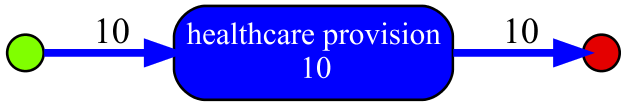
\includegraphics[width=0.45\textwidth]{AmbulatoriInductiveVisualMinerYoungs4301}
\caption{Urologia ($\leq$25 years)}
\end{figure}\\
Moreover, patients belonging from [\ref{Word:young}] go in both outpatient clinics `\textit{5801}' (Gastroenterologia) and `\textit{0901}' (Chirurgia generale) with medical prescriptions compiled only by `\textit{1}' (medico di medicina generale). For patients belonging from [\ref{Word:old}] there are also cases of medical prescriptions compiled by `\textit{2}' (medico specialista dipendente da struttura pubblica).\\
Looking at the performance perspective, in particular at the \textit{sojourn time} point of view, we obtained:
\begin{figure} [htbp]
\begin{minipage}[t]{0.5\textwidth}
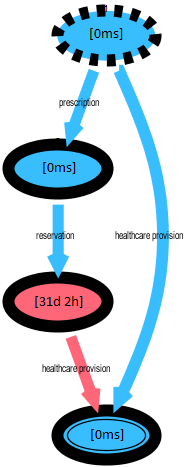
\includegraphics[width=0.5\textwidth]{AmbulatorioSojournYoungs}
\caption{Transition system ($\leq$25 years)}
\end{minipage}
\begin{minipage}[t]{0.5\textwidth}
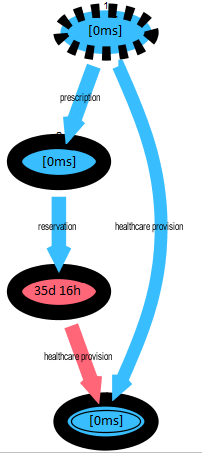
\includegraphics[width=0.55\textwidth]{AmbulatorioSojournOlds}
\caption{Transition system ($>$25 years)}
\end{minipage}
\end{figure}\\
At first glance, looking at the two transition systems we can see that the states associated with activities belonging to the cluster [\ref{Word:old}] have a border ticker than the states associated with activities belonging to the cluster [\ref{Word:young}], since the cluster [\ref{Word:young}] contains a number of patient's cases strictly lower than the cluster [\ref{Word:old}]. The same argument applies to arcs. Moreover, we can see that the most of time, for both the clusters [\ref{Word:young}] and [\ref{Word:old}], is spent on the activity `\textit{reservation}' where a patient is waiting for the healthcare provision. % the average sojourn time for this activity is 31 days 1 hour for patients belonging to [\ref{Word:young}] and 35 days 17 hours for patients belonging to [\ref{Word:old}].
The avg sojourn time of both the clusters is equal (more or less) to the one of the blueprint.
\clearpage
\noindent
\section{Pronto soccorso dataset}\label{analysis:2}
The \setword{blueprint}{Word:prontosoccorsoblueprint} in terms of process model is the following:
\begin{figure} [htbp]
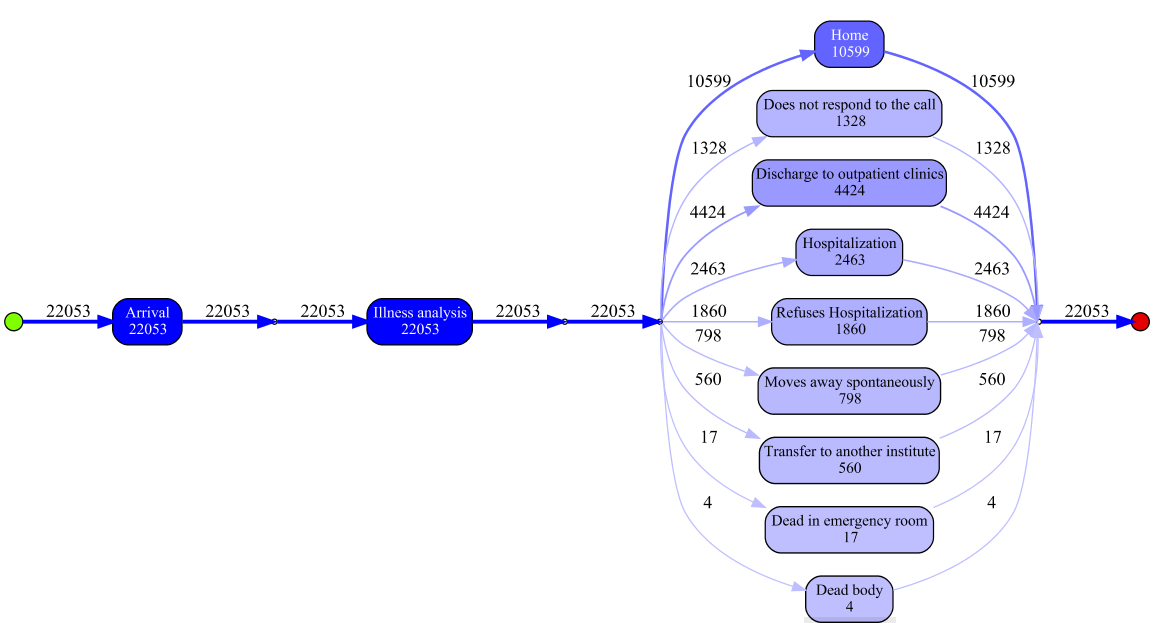
\includegraphics[width=0.75\textwidth, keepaspectratio]{ProntoSoccorsoInductiveVisualMiner}
\caption{Clinical path (Totality of patients)}
\end{figure}\\
Looking at the figure, we can see that a patient arrives in emergency room, then performs the problem diagnosis. From here, the patient can have several outcomes. It figures out that the majority of patients are sent home after the illness analysis. From the organizational point of view, the \setword{social network}{Word:prontosoccorsosocialnetwork} derived is as follows:
\begin{figure} [htbp]
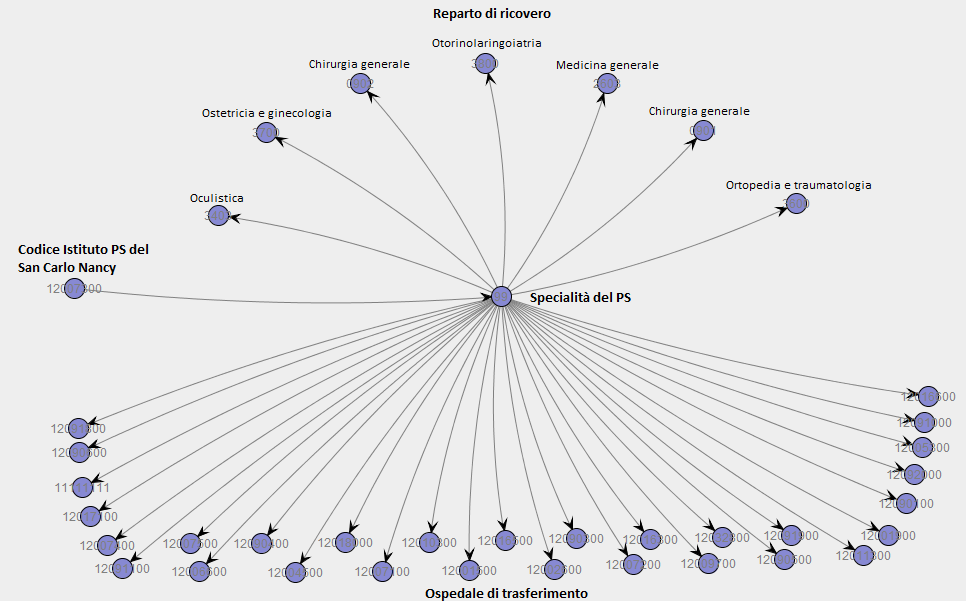
\includegraphics[width=0.7\textwidth, keepaspectratio]{ProntoSoccorsoSocialNetwork}
\caption{Social network (Totality of patients)}
\end{figure}\\
From the social network points out a patient go in emergency room, that is, the one coded with `\textit{12007300}' (San Carlo Nancy emergency room); then he is assigned to emergency room specialty `\textit{99}' and from here he can be either transferred to another Institute or to another hospitalization ward.
\clearpage
\noindent
On the other hand, the transition system, under the \textit{sojourn time} point of view is the following:
\begin{figure} [htbp]
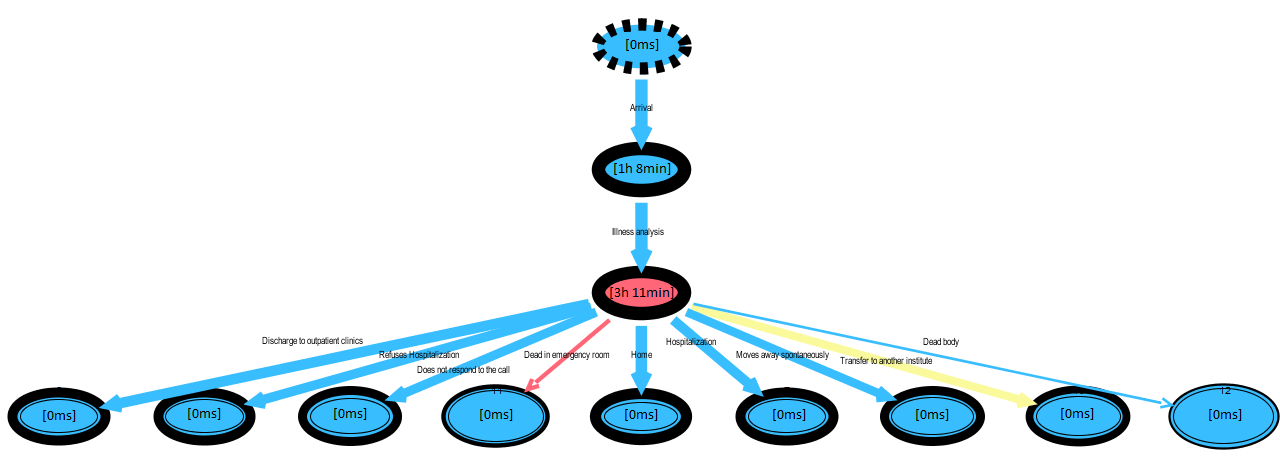
\includegraphics[width=\textwidth, keepaspectratio]{ProntoSoccorsoTransitionSystemSojourn}
\caption{Transition System (Totality of patients)}
\end{figure}\\
We can see that the most of time is spent on the activity `\textit{illness analysis}'. Since, the standard deviation diverges from the different average times, meaning that the patients are spread out over a wide range of time,then the mean is not significant at all. For this reason, we have repeated the same analysis for different cluster of patients. We started with both the clusters of foreign [\ref{Word:foreign}] and the italian [\ref{Word:italian}] patients, obtaining the following process models:
\begin{figure} [htbp]
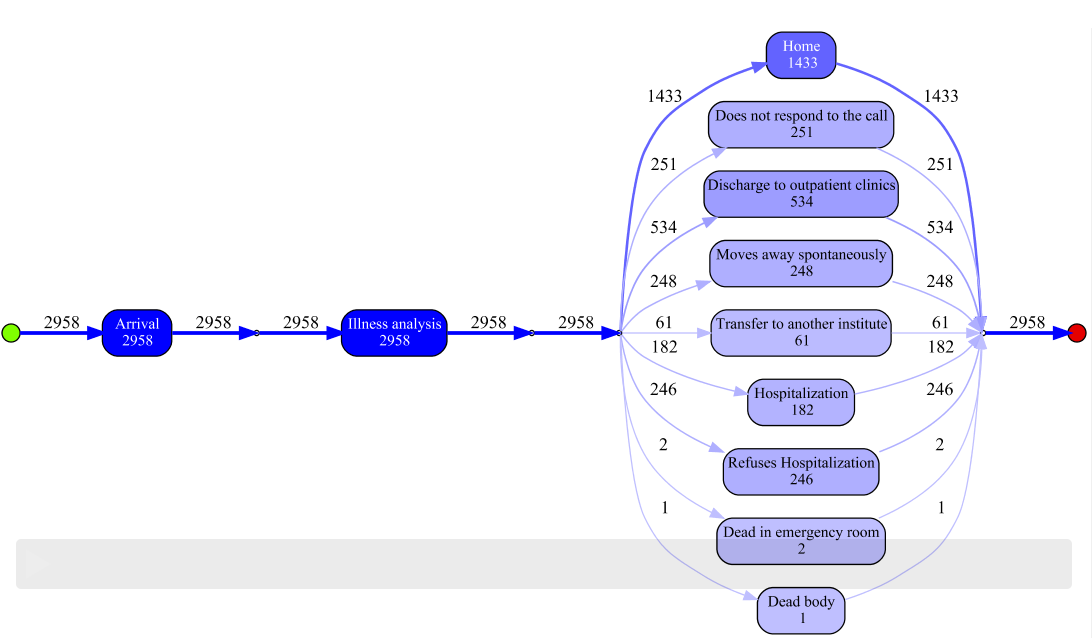
\includegraphics[width=\textwidth , keepaspectratio]{ProntoSoccorsoInductiveVisualMinerForeigns}
\caption{Clinical path (Foreign patients)}
\end{figure}
\clearpage
\noindent
\begin{figure} [htbp]
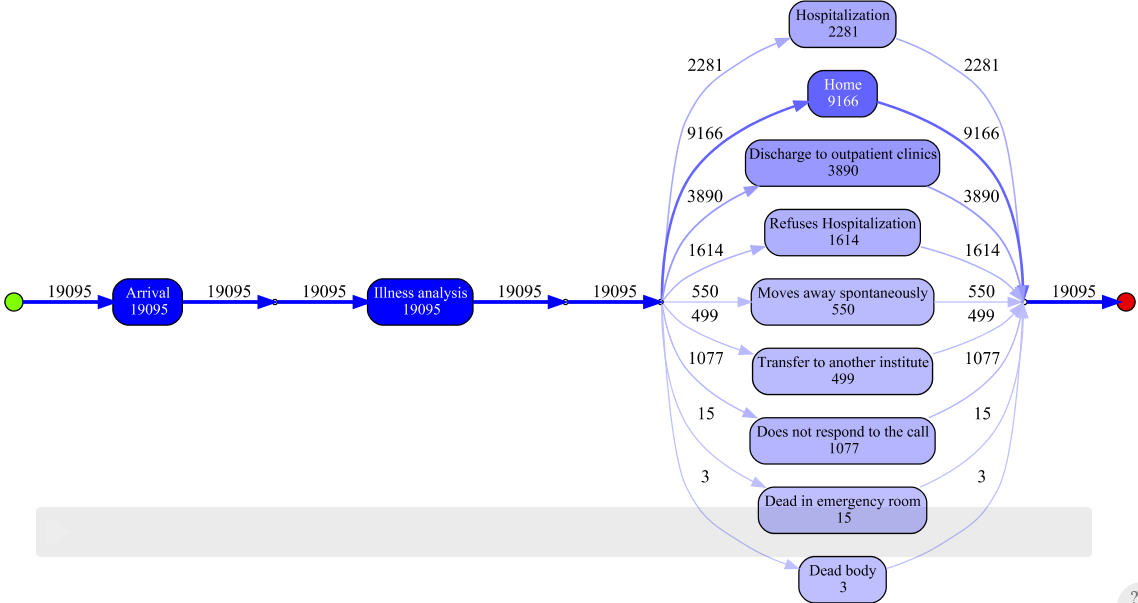
\includegraphics[width=\textwidth , keepaspectratio]{ProntoSoccorsoInductiveVisualMinerItalians}
\caption{Clinical path (Italian patients)}
\end{figure}\\
Both the process models are identical to the \ref{Word:prontosoccorsoblueprint}, the only difference is on the number of process executions (2958 for [\ref{Word:foreign}] and 19095 for [\ref{Word:italian}]). Furthermore, looking at both the figures, we can see that the most of both foreign and italian patients after performed the illness analysis are sent home. From the organizational point of view, the social networks derived from both the clusters [\ref{Word:foreign}] and [\ref{Word:italian}] are as follows:
\begin{figure} [htbp]
\begin{minipage}[t]{0.5\textwidth}
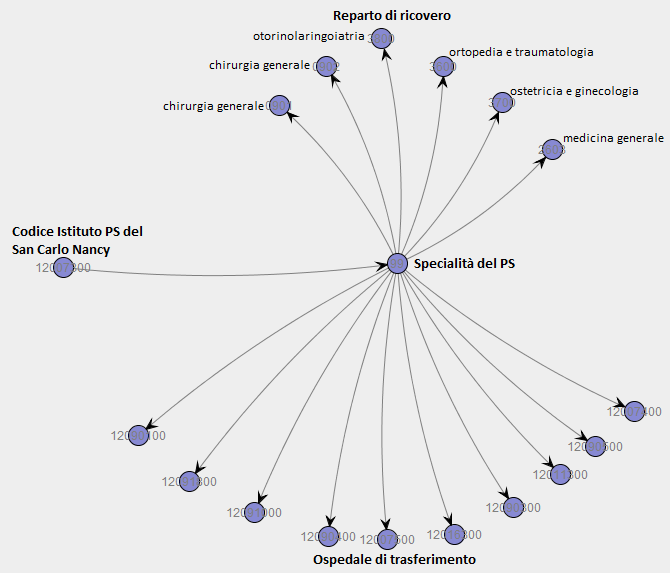
\includegraphics[width=\textwidth , keepaspectratio]{ProntoSoccorsoHoWForeigns}
\caption{Social network (Foreign patients)}
\end{minipage}
\begin{minipage}[t]{0.5\textwidth}
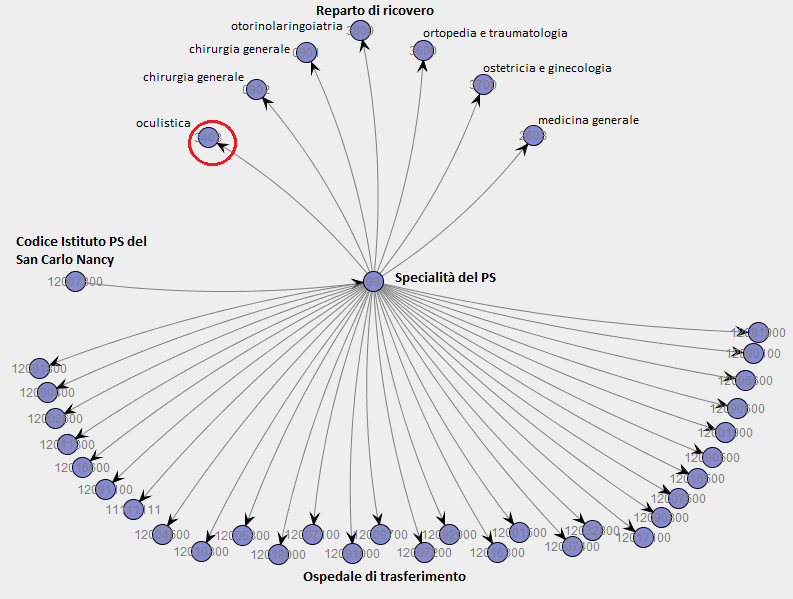
\includegraphics[width=1.125\textwidth , keepaspectratio]{ProntoSoccorsoHoWItalians}
\caption{Social network (Italian patients)}
\end{minipage}
\end{figure}
\newline
\noindent
Looking at the pictures, the social networks of the patients belonging from both the clusters [\ref{Word:foreign}] and [\ref{Word:italian}] are quite different. The main difference, which it’s pretty obvious, is that the number of resources involved in the cluster of the italian patients is more grater than the number of resources involved in the cluster of the foreign patients. In particular, italian patients are transferred in a greater number of Institutes. Moreover, there is the hospitalization ward `\textit{3403}' (oculistica) belonging only to the cluster of italian patients. The transition systems, on the \textit{sojourn time} point of view, are:
\begin{figure} [h]
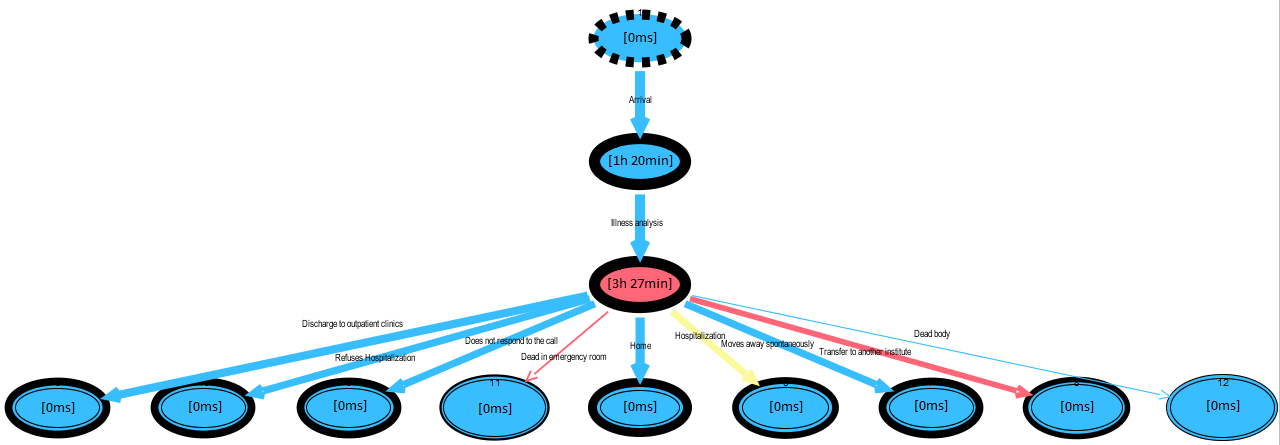
\includegraphics[width=\textwidth]{ProntoSoccorsoSojournForeigns}
\caption{Transition system (Foreign patients)}
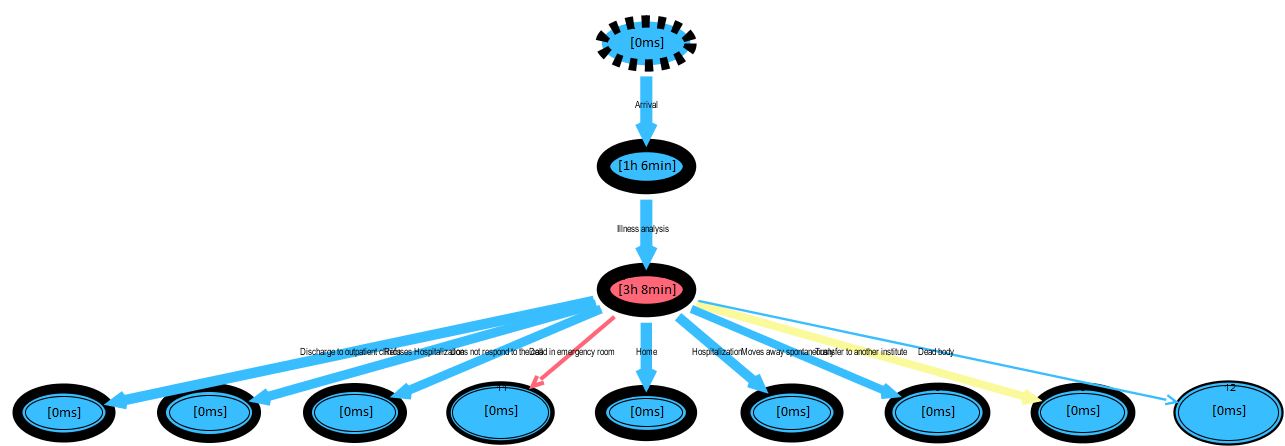
\includegraphics[width=\textwidth]{ProntoSoccorsoSojournItalians}
\caption{Transition system (Italian patients)}
\end{figure} \newline
At first glance, looking at the two transition systems we can see that the states associated with activities belonging to the cluster [\ref{Word:italian}] have a border ticker than the states associated with activities belonging to the cluster [\ref{Word:foreign}], since the cluster [\ref{Word:foreign}] contains a number of patient's cases strictly lower than the cluster [\ref{Word:italian}]. The same argument applies to arcs. Moreover, we can see that the most of time, for both the clusters [\ref{Word:foreign}] and [\ref{Word:italian}] is spent on the activity `\textit{illness analysis}' where the patient is waiting for the result of the diagnosis. The avg sojourn time of both the clusters is equal (more or less) to the one of the blueprint. Then, we have considered both the clusters of patients with an age lower or equal than 25 years (resident in Latium) [\ref{Word:young}] and the cluster of patients with an age greater than 25 years (resident in Latium) [\ref{Word:old}]. 
\clearpage
\noindent
The process models obtained are the following:
\begin{figure} [htbp]
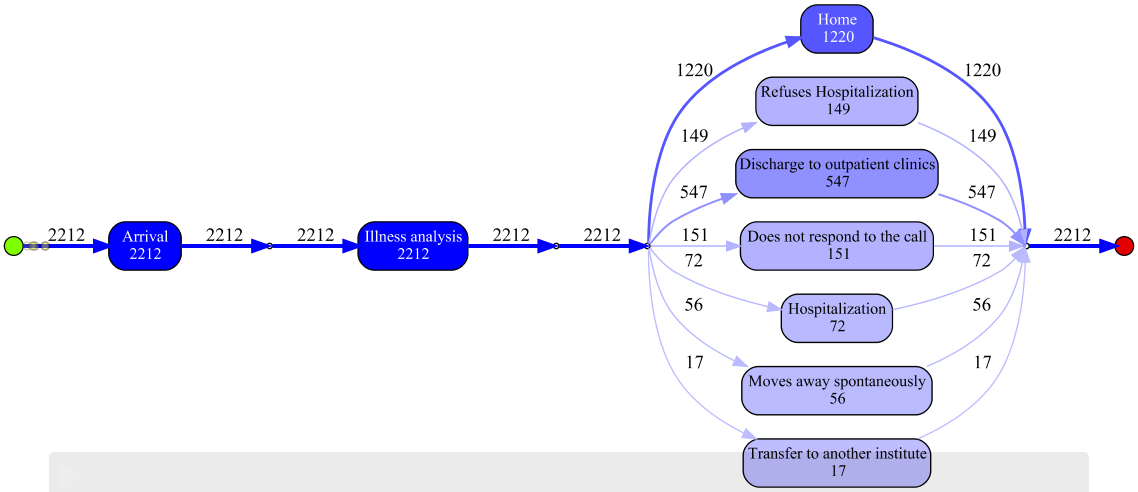
\includegraphics[width=\textwidth, keepaspectratio]{ProntoSoccorsoInductiveVisualMinerYoungs}
\caption{Clinical path ($\leq$25 years)}
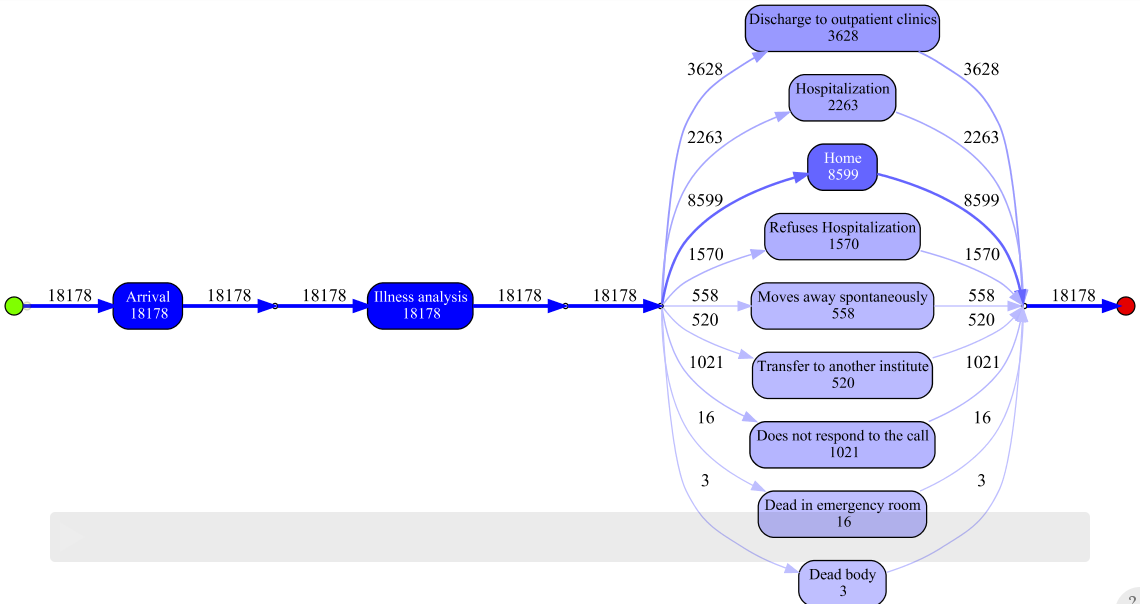
\includegraphics[width=\textwidth, keepaspectratio]{ProntoSoccorsoInductiveVisualMinerOlds}
\caption{Clinical path ($>$25 years)}
\end{figure}
Looking at the process model we can see that the patients with an age lower or equal than 25 years (resident in Latium) [\ref{Word:young}] does not have the activities: `\textit{dead body}' and `\textit{dead in emergency room}', with respect to the cluster of patients with an age greater than 25 years (resident in Latium) [\ref{Word:old}]. However, the behaviour of the patients belonging to these two clusters is pretty equal; also the most frequent path is the same: `\textit{arrival}' $\Rightarrow$ `\textit{illness analysis}' $\Rightarrow$ `\textit{home}'.
\clearpage
\noindent
The derived social networks for both [\ref{Word:young}] and [\ref{Word:old}] are:

\begin{figure} [htbp]
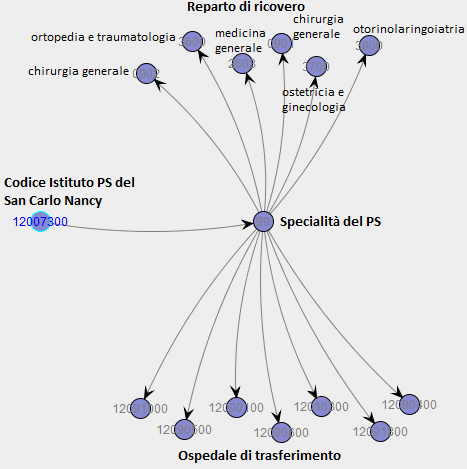
\includegraphics[width=0.75\textwidth, keepaspectratio]{ProntoSoccorsoHoWYoungs}
\caption{Social network ($\leq$25 years)}
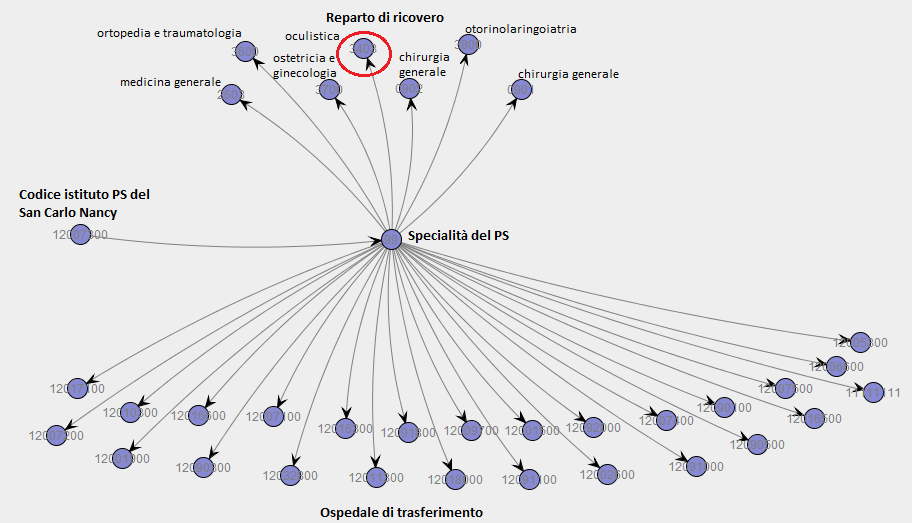
\includegraphics[width=0.75\textwidth, keepaspectratio]{ProntoSoccorsoHoWOlds}
\caption{Social network ($>$25 years)}
\end{figure}
\noindent
The main difference, which it’s pretty obvious, is that the number of resources involved in the cluster of patients with an age greater than 25 years (resident in Latium) [\ref{Word:old}] is more greater than the number of resources involved in the cluster of patients with an age lower or equal than 25 years (resident in Latium) [\ref{Word:young}]. In particular, the patients of the cluster [\ref{Word:old}] are transferred in a greater number of Institutes. Furthermore, there is the hospitalization ward `\textit{3403}' (oculistica) belonging only to the cluster [\ref{Word:old}]. The transition systems, on the \textit{sojourn time} point of view, are:
\begin{figure} [htbp]
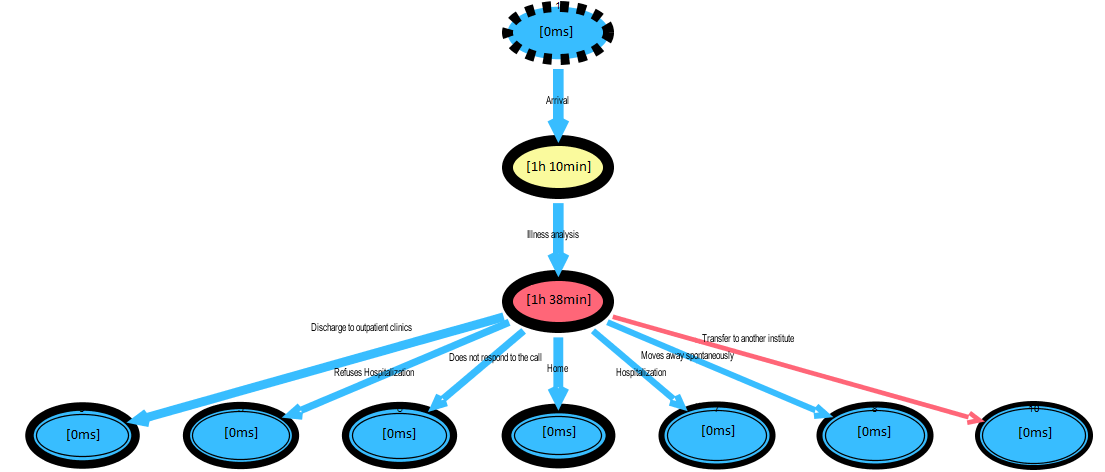
\includegraphics[width=\textwidth , keepaspectratio]{ProntoSoccorsoSojournYoungs}
\caption{Transition system ($\leq$25 years)}
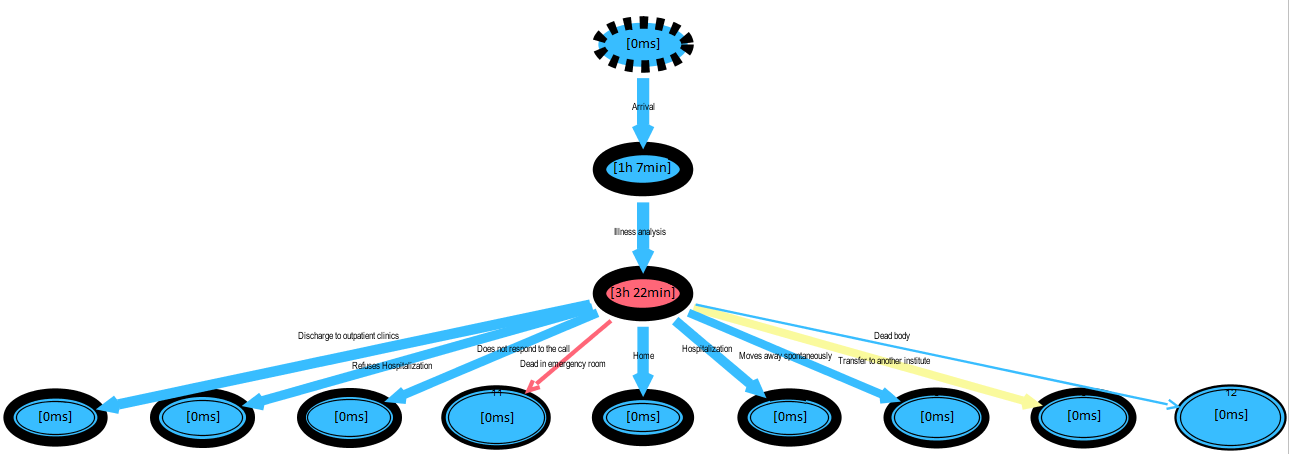
\includegraphics[width=\textwidth , keepaspectratio]{ProntoSoccorsoSojournOlds}
\caption{Transition system ($>$25 years)}
\end{figure} \\
At first glance, looking at the two transition systems we can see that both states and arcs associated with activities belonging to the cluster [\ref{Word:old}] have a border ticker than the states associated with activities belonging to the cluster [\ref{Word:young}] (the reason is always the same). Moreover, we can see that the most of time, for both the clusters [\ref{Word:young}] and [\ref{Word:old}] is spent on the activity `\textit{illness analysis}' where the patient is waiting for the result of the diagnosis.
\clearpage
\section{Ricoveri dataset}\label{analysis:3}
The \setword{blueprint}{Word:ricoveriblueprint} in terms of process model is the following:
\begin{figure} [htbp]
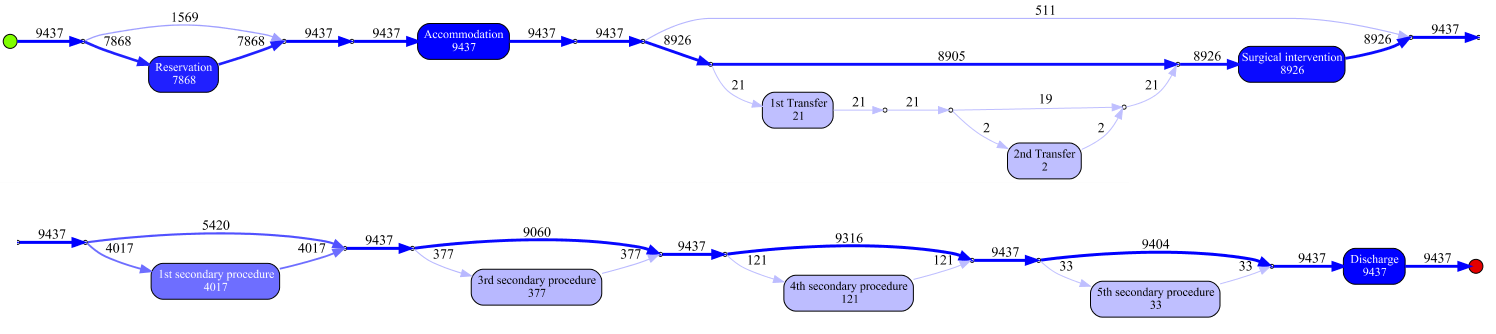
\includegraphics[width=\textwidth]{RicoveriProcessModel2}
\caption{Clinical path (Totality of Patients)}
\end{figure}\\
Looking at the figure, we can see that a patient can ask for a reservation, then he/she is accommodated in order to perform the surgical intervention. Notice that, before the surgical intervention, a patient can be transferred from a hospitalization ward to another one. However, the transfers could happen also after the surgical intervention and between the secondary procedure. This behavior is not captured by the process model, and therefore it contains deviations with respect to event log. After the surgical intervention a patient can be either directly discharged or submitted through a chain of secondary procedures that will end with the discharge
of the patient. Notice that a patient may skip the surgical intervention.. From the organizational point of view, the derived \setword{social network}{Word:ricoverisocialnetwork} is the following:
\begin{figure} [htbp]
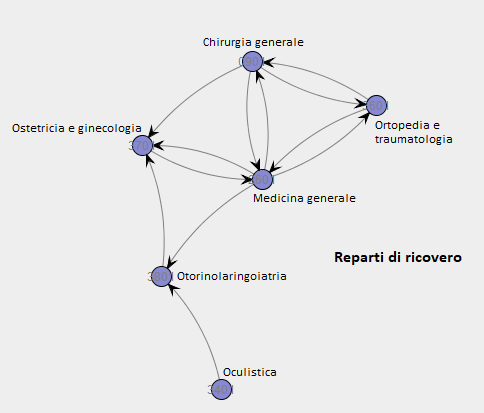
\includegraphics[width=0.75\textwidth]{RicoveriSocialNetwork}
\caption{Social Network (Totality of Patients)}
\end{figure}\\
The social network shows how the different hospitalization wards interact between each other. The semantic of the social network is the following: an arc from a hospitalization ward `\textit{x}' to another hospitalization ward `\textit{y}' means that exist at least a patient transferred from `\textit{x}' to `\textit{y}'. For example, if we take in consideration the hospitalization ward `\textit{3401}' (oculistica), there is at least a patient that is transferred to the hospitalization wards `\textit{3801}' (otorinolaringoiatria).\\
Regarding the performance perspective we have obtained:
\begin{figure} [htbp]
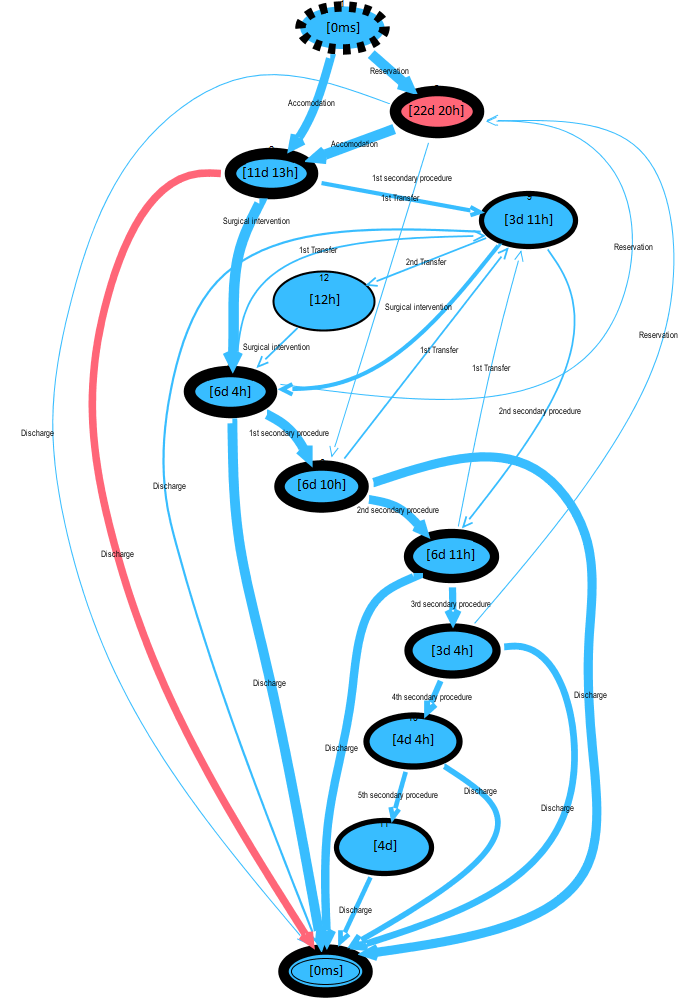
\includegraphics[width=0.85\textwidth , keepaspectratio]{RicoveriTransitionSystemSojourn}
\caption{Transition system (Totality of Patients)}
\end{figure}
\clearpage
\noindent
We can see that the most of time, from the \textit{sojourn time} point of view, is spent on the activity `\textit{reservation}' where the patient is waiting for the accomodation to be hospitalized. Also the transition from the accomodation state to the discharge state takes a very long time. The standard deviation of these different average times is very high, meaning that the patients are spread out over a wide range of time, therefore the mean is not significant at all. There are patients that behaves different from other patients. For this reason we have split in different clusters the set of patients in order to discover interesting properties. Since, the primary of a hospitalization ward has the goal to minimize the time of the overall hospitalization procedure of a patient, we wanted to understand the bottleneck activities which slow down the entire hospitalization procedure. Therefore, we have performed an ad-hoc analysis for the patients who performed only the main surgical intervention without any secondary procedure and transfers to other hospitalization wards (in order to make uniform the data for the analysis). Since, we're interested in three particular hospitalization wards we have defined three different cluster of patients:
\begin{itemize}
\item patients hospitalized in the hospitalization ward `\textit{0901}' (\setword{chirurgia generale}{Word:chirurgiagenerale}) 
\item patients hospitalized in the hospitalization ward `\textit{2601}' (\setword{medicina generale}{Word:medicinagenerale})
\item patients hospitalized in the hospitalization ward `\textit{3601}' (\setword{ortopedia e traumatologia}{Word:ortopediatraumatologia})
\end{itemize}
for each cluster we have looked on how the patients are distributed over the time and we selected a 5\% of patients with the lowest time duration of hospitalization procedure and a 5\% of patients with the highest time duration ofhospitalization procedure. From this two subclusters we discovered process models, social networks and transition systems (looking only at the sojourn time point of view).
\newline
We started the analysis with the cluster of patients hospitalized in the hospitalization ward \ref{Word:chirurgiagenerale}. The process model obtained is:
\begin{figure} [htbp]
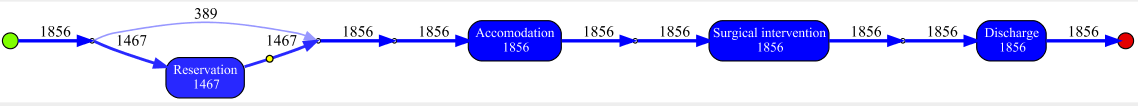
\includegraphics[width=\textwidth , keepaspectratio]{RicoveriInductiveVisualMiner0901}
\caption{Chirurgia generale}
\end{figure}
\newline
From the picture, points out, the most of patients ask for a reservation instead of being directly accomodated. Regarding the social network, we got trivially, a social network made up by only one hospitalization ward, since we're considering only patients of `\textit{0901}' (chirurgia generale): 
\begin{figure} [htbp]

\includegraphics[width=0.15\textwidth , keepaspectratio]{RicoveriSocialNetwork0901}
\caption{Chirurgia generale}
\end{figure}
\clearpage
\noindent
The derived transition system (sojourn time point of view) is:
\begin{figure} [htbp]
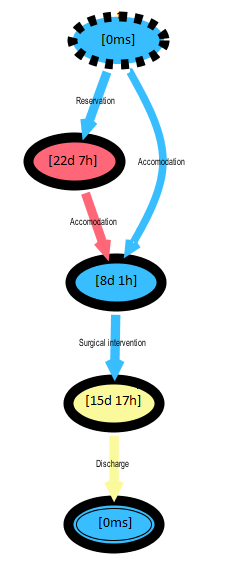
\includegraphics[width=0.25\textwidth , keepaspectratio]{RicoveriTransitionSystemSojourn0901}
\caption{Chirurgia generale}
\end{figure}\\
From the transition system points out that the patients take a very long time both to be accomodated and to be discharged. Then, we split the cluster \ref{Word:chirurgiagenerale} in two subclusters and we compared them between each other. For doing that, we first looked at the distribution of patients belonging to that cluster:
\begin{figure} [htbp]
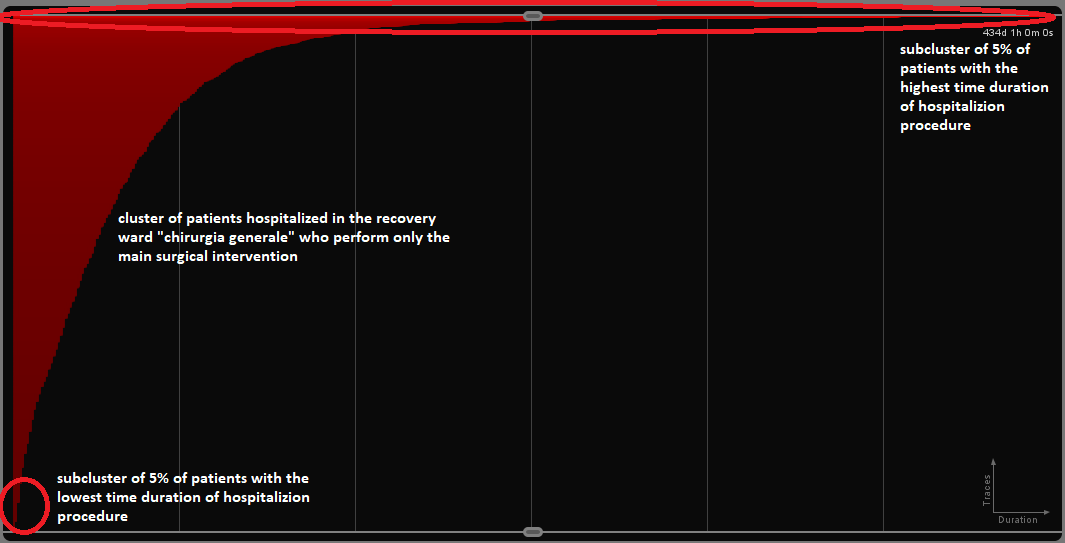
\includegraphics[width=0.75\textwidth , keepaspectratio]{RicoveriChart}
\caption{Distribution of patients based on time duration}
\end{figure}\\
The Y-axis represents the patients and the X-axis represent the time duration. The 5\% of patients with the lowest time duration of hospitalization procedure is lozalized in the bottom zone in red, instead the 5\% of patients with the highest time duration of hospitalization procedure is lozalized in the top zone in red. The process model obtained from the subclusters are the following:
\begin{figure} [htbp]
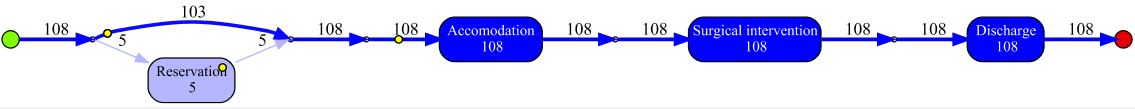
\includegraphics[width=\textwidth , keepaspectratio]{RicoveriInductiveVisualMiner0901Fast}
\caption{5\% of patients with the lowest time duration of hospitalization (Chirurgia generale)}
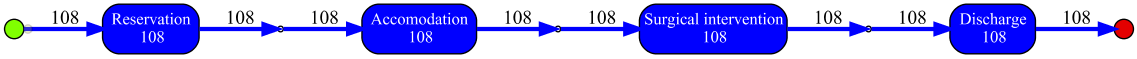
\includegraphics[width=\textwidth , keepaspectratio]{RicoveriInductiveVisualMiner0901Slow}
\caption{5\% of patients with the highest time duration of hospitalization (Chirurgia generale)}
\end{figure}\\
The difference that points out is on the most frequent path taken by the patients belonging to the two different subclusters. All the 5\% of patients with the highest time duration of hospitalization (chirurgia generale) ask for a reservation, instead, the 5\% of patients with the slowest time duration of hospitalization (chirurgia generale) are directly accomodated for hospitalization. The social networks obtained are the same as the one obtained for the main cluster \ref{Word:chirurgiagenerale} and for this reason we won't show them. Instead, it's important to show the transition systems, on the sojourn time point of view:
\begin{figure} [htbp]
\begin{minipage}[t]{0.3\textwidth}
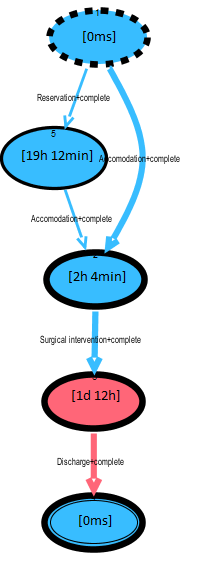
\includegraphics[width=0.7\textwidth]{RicoveriTransitionSystemSojourn0901Fast}
\caption{5\% of patients with the lowest time duration of hospitalization (Chirurgia generale)}
\end{minipage}
\begin{minipage}[t]{0.32\textwidth}
\includegraphics[width=0.5\textwidth]{RicoveriTransitionSystemSojourn0901Slow}
\caption{5\% of patients with the highest time duration of hospitalization (Chirurgia generale)}
\end{minipage}
\end{figure}
\clearpage
\noindent
The bottleneck is on the time that a patient is waiting for the accomodation (look at the red arrow). Moreover, also the time spent from the surgical intervention to the discharge of the patient is high (look at the yellow arrow). For the subclusters derived from \ref{Word:chirurgiagenerale}, we concluded:
\begin{itemize}
\item the hospitalization procedure is quick when the patients didn't ask for a reservation and they are directly accomodated for being hospitalized.
\item the hospitalization procedure is mainly slowed down by the waiting time of the patients asking for the reservation but also on the time difference between the surgical intervention and the discharge of the patient (the primary of a hospitalization ward is more interested to minimize this time).
\end{itemize}
The procedure for the cluster \ref{Word:medicinagenerale} is impossible to be applied due to the small number of patients who performed only the main surgical intervention without transfers and secondary procedures (59 case IDs). On the other hand, we were able to analyze the cluster \ref{Word:ortopediatraumatologia}. The process model obtained is:
\begin{figure} [htbp]
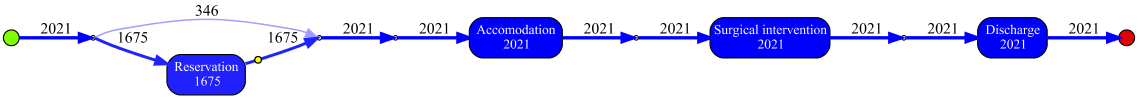
\includegraphics[width=\textwidth , keepaspectratio]{RicoveriInductiveVisualMiner3601}
\caption{Ortopedia e traumatologia}
\end{figure}
\newline
From the picture, points out, the majority of patients belonging to \ref{Word:ortopediatraumatologia} asks for a reservetion in order to be accomodated for the hospitalization instead of being directly accomodated. Regarding the social network, we got trivially, a social network made up by only one hospitalization wards, since we're considering only patients of `\textit{3601}' (ortopedia e traumatologia): 
\begin{figure} [htbp]
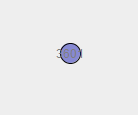
\includegraphics[width=0.3\textwidth , keepaspectratio]{RicoveriSocialNetwork3601}
\caption{Ortopedia e traumatologia}
\end{figure}
\clearpage
\noindent
The derived transition system (on the sojourn time point of view) is:
\begin{figure} [htbp]
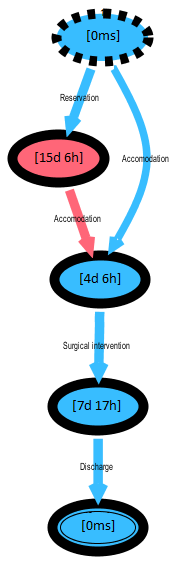
\includegraphics[width=0.22\textwidth]{RicoveriTransitionSystemSojourn3601}
\caption{Ortopedia e traumatologia}
\end{figure}\\
Then we have split the cluster \ref{Word:ortopediatraumatologia} in two subclusters and we compared them between each other. The distribution of patients belonging to that cluster is the following:
\begin{figure} [htbp]
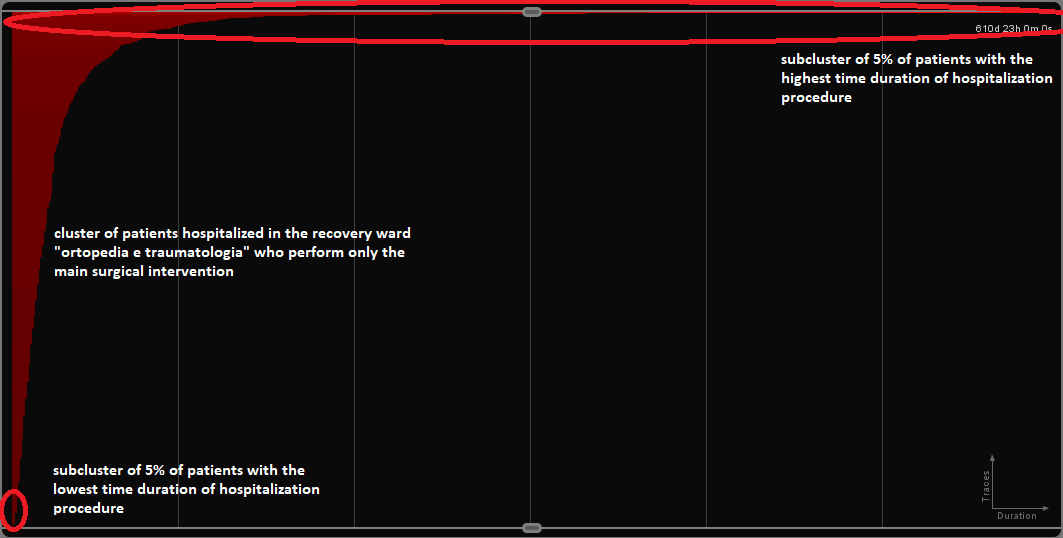
\includegraphics[width=0.75\textwidth]{RicoveriChart3}
\caption{Distribution of patients based on time duration}
\end{figure}\\
The Y-axis represents the patients and the X-axis represent the time duration. The 5\% of patients with the lowest time duration of hospitalization procedure is lozalized in the bottom zone in red, instead the 5\% of patients with the highest time duration of hospitalization procedure is lozalized in the top zone in red. 
\clearpage
\noindent
The process models obtained are the following:
\begin{figure} [htbp]
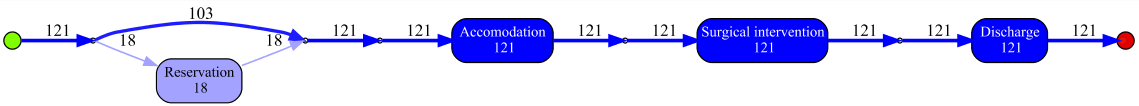
\includegraphics[width=\textwidth]{RicoveriInductiveVisualMiner3601Fast}
\caption{5\% of patients with the lowest time duration of hospitalization (Ortopedia e traumatologia)}
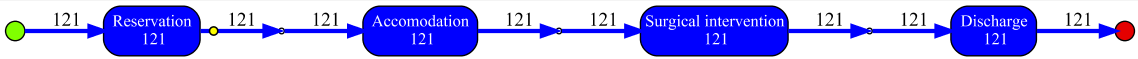
\includegraphics[width=\textwidth]{RicoveriInductiveVisualMiner3601Slow}
\caption{5\% of patients with the highest time duration of hospitalization (Ortopedia e traumatologia)}
\end{figure}\\
The difference that points out is on the most frequent path taken by the patients belonging to the two different subclusters. The overall 5\% of patients with the highest time duration of hospitalization (ortopedia e traumatologia) ask for a reservation, instead, the 5\% of patients with the slowest time duration of hospitalization (ortopedia e traumatologia) is directly accomodated for hospitalization. The social networks obtained are the same as the one obtained for the main cluster \ref{Word:ortopediatraumatologia} and for this reason we won't show them. Instead, it's important to show the transition systems, on the sojourn time point of view:
\begin{figure} [htbp]
\begin{minipage}[t]{0.3\textwidth}
\includegraphics[width=0.7\textwidth]{RicoveriTransitionSystemSojourn3601Fast}
\caption{5\% of patients with the lowest time duration of hospitalization (Ortopedia e traumatologia)}
\end{minipage}
\begin{minipage}[t]{0.3\textwidth}
\includegraphics[width=0.5\textwidth]{RicoveriTransitionSystemSojourn3601Slow}
\caption{5\% of patients with the highest time duration of hospitalization (Ortopedia e traumatologia)}
\end{minipage}
\end{figure}\\
The bottleneck is on the time that a patient is waiting for the accomodation (look at the red arrow). Therefore, for the subclusters derived from \ref{Word:ortopediatraumatologia}, we concluded that the hospitalization procedure is mainly slowed down by the waiting time of the patients asking for the reservation of the hospitalization.\\
After did this in-depth analysis, we considered the set of clusters: [\ref{Word:foreign}], [\ref{Word:italian}], [\ref{Word:young}],  [\ref{Word:old}]. The process models obtained for the clusters [\ref{Word:foreign}] and [\ref{Word:italian}] are:
\begin{figure} [htbp]
\includegraphics[width=\textwidth]{RicoveriInductiveVisualMinerForeigns}
\caption{Clinical path (Foreign patients)}
\includegraphics[width=\textwidth]{RicoveriInductiveVisualMinerItalian}
\caption{Clinical path (Italian patients)}
\end{figure}\\
Both the process models are identical to the blueprint (in terms of behaviour of the patients), the only difference is on the number of process executions (264 for [\ref{Word:foreign}] and 9173 for [\ref{Word:italian}]). Furthermore, looking at both the figures, we can see that the majority of both foreign and italian patients ask for a reservation, then they are accomodated for being hospitalized and after the surgical intervention they are discharged. On the other hand, the derived social network for both the clusters of foreign [\ref{Word:foreign}] and italian patients [\ref{Word:italian}] are:
\begin{figure} [htbp]
\begin{minipage}[t]{0.5\textwidth}
\includegraphics[width=0.8\textwidth , keepaspectratio]{RicoveriSocialNetworkForeigns}
\caption{Social network (Foreign patients)}
\end{minipage}
\begin{minipage}[t]{0.5\textwidth}
\includegraphics[width=\textwidth , keepaspectratio]{RicoveriSocialNetworkItalians}
\caption{Social network (Italian patients)}
\end{minipage}
\end{figure}
\clearpage
\noindent
From the social network of the cluster of foreign patients [\ref{Word:foreign}] we can see that the hospitalization ward `\textit{3401}'  is not involved in any social relations, meaning that the patients hospitalized in `\textit{3401}' (oculistica) won't be transferred in any other hospitalization wards. Instead, the social network of the cluster of italian patients [\ref{Word:italian}] is more or less equal to the \ref{Word:ricoverisocialnetwork} of the blueprint: it contains the same number of resources but the social relations are a subset. \\
The transition systems, on the \textit{sojourn time} point of view, are:
\begin{figure} [htbp]
\begin{minipage}[t]{0.4\textwidth}
\includegraphics[width=\textwidth]{RicoveriTransitionSystemSojournForeigns}
\caption{Transition system (Foreign patients)}
\end{minipage}
\begin{minipage}[t]{0.6\textwidth}
\includegraphics[width=\textwidth]{RicoveriTransitionSystemSojournItalians}
\caption{Transition system (Italian patients)}
\end{minipage}
\end{figure}\\
Looking at both the transition systems we can see the bottleneck is on the activity `\textit{reservation}'. We can see also that states and arcs associated with the cluster of italian patients are more thick than the states and arcs associated with the cluster of foreign patients, since the number of foreign patients is strictly lower than the number of italian patients.
\clearpage
\noindent
At last, we have repeated the same steps for both the clusters [\ref{Word:young}], [\ref{Word:old}]. The derived process models are:
\begin{figure} [htbp]
\includegraphics[width=\textwidth]{RicoveriInductiveVisualMinerYoungs}
\caption{Clinical path ($\leq$25 years)}
\includegraphics[width=\textwidth]{RicoveriInductiveVisualMinerOlds}
\caption{Clinical path ($>$25 years)}
\end{figure}\\
The process models are similar but there are slightly differences: patients belonging to the cluster [\ref{Word:young}] performs only the `\textit{1st transfer}' and not the `\textit{2nd transfer}'                                                                                                                                                                                                                                                                                                                                                                                                                                                                                                                                                                 . Note that the process model for [\ref{Word:old}] presents deviations regarding transfers, since they can happen also after the surgical intervention. Loooking at the process executions (1399 for [\ref{Word:young}] and 8038 for [\ref{Word:old}]) we can see that the number of patients belonging to [\ref{Word:young}] are strictly lower than the number of patients belonging to [\ref{Word:old}].\\
The derived social network for both the clusters [\ref{Word:young}] and [\ref{Word:old}] are:
\begin{figure} [htbp]
\begin{minipage}[t]{0.4\textwidth}
\includegraphics[width=\textwidth]{RicoveriSocialNetworkYoungs}
\caption{Social network ($\leq$25 years)}
\end{minipage}
\begin{minipage}[t]{0.6\textwidth}
\includegraphics[width=0.9\textwidth]{RicoveriSocialNetworkOlds}
\caption{Social network ($>$25 years)}
\end{minipage}
\end{figure}\\
From the social network of patients belonging to the cluster [\ref{Word:young}] the resources involved in social relations are both `\textit{0901}' (chirurgia generale) and `\textit{2601}' (medicina generale), meaning that patients are transferred from the hospitalization ward `\textit{0901}' to `\textit{2601}' and viceversa. Instead, the social network of patients belonging to the cluster [\ref{Word:old}] is equal to the \ref{Word:ricoverisocialnetwork} of the blueprint. The transition systems, on the \textit{sojourn time} point of view, are:
\begin{figure} [htbp]
\begin{minipage}[t]{0.3\textwidth}
\includegraphics[width=\textwidth]{RicoveriTransitionSystemSojournYoungs}
\caption{Transition system ($\leq$25 years)}
\end{minipage}
\begin{minipage}[t]{0.55\textwidth}
\includegraphics[width=\textwidth]{RicoveriTransitionSystemSojournOlds}
\caption{Transition system ($>$25 years)}
\end{minipage}
\end{figure}\\
Looking at both the transition systems we can see the bottleneck is on the activities `\textit{reservation}' and `\textit{accomodation}' (only for patients belonging to [\ref{Word:young}]). We can see also that states and arcs associated with the cluster [\ref{Word:old}] are more thick than the states and arcs associated with the cluster of [\ref{Word:young}], since the number of patients with an age lower or equal than 25 years (resident in Latium) is strictly lower than the number of patients with an age greater than 25 years (resident in Latium).
\clearpage
\noindent
\section{Conclusions} \label{conclusions}
In this paper, we have focused on the applicability of process mining in the healthcare domain. We have focused on the analysis of the results obtained for our case study. In particular, we have used the raw datasets of \hospital in order to discover several non-trivial care processes, social networks and transition systems by using the ProM framework. Thus, we have shown that is possible to mine complex hospital processes giving insights into the process, that is, with existing techniques we were able to derive an understandable model for all the patients. In particular, we focused on obtaining insights into the careflow by looking at
the control flow perspective and presenting the results showing the differences between the process models of the different cluster of patients. We have also look on the organizational perspective of the process models describing how the resources can communicate among them. In conclusion, we have also looked on the performance perspective of process models, analyzing the transition systems obtained from relevant event logs.

\begin{comment}
% For one-column wide figures use
\begin{figure}
% Use the relevant command to insert your figure file.
% For example, with the graphicx package use
  \includegraphics{example.eps}
% figure caption is below the figure
\caption{Please write your figure caption here}
\label{fig:1}       % Give a unique label
\end{figure}
%
% For two-column wide figures use
\begin{figure*}
% Use the relevant command to insert your figure file.
% For example, with the graphicx package use
  \includegraphics[width=0.75\textwidth]{example.eps}
% figure caption is below the figure
\caption{Please write your figure caption here}
\label{fig:2}       % Give a unique label
\end{figure*}
%
% For tables use
\begin{table}
% table caption is above the table
\caption{Please write your table caption here}
\label{tab:1}       % Give a unique label
% For LaTeX tables use
\begin{tabular}{lll}
\hline\noalign{\smallskip}
first & second & third  \\
\noalign{\smallskip}\hline\noalign{\smallskip}
number & number & number \\
number & number & number \\
\noalign{\smallskip}\hline
\end{tabular}
\end{table}
\end{comment}

%\begin{acknowledgements}
%If you'd like to thank anyone, place your comments here
%and remove the percent signs.
%\end{acknowledgements}
\nocite{*}
% BibTeX users please use one of
\bibliographystyle{bise}      % Bise style
%\bibliographystyle{spbasic}      % basic style, author-year citations
%\bibliographystyle{spmpsci}      % mathematics and physical sciences
%\bibliographystyle{spphys}       % APS-like style for physics
\bibliography{bibliography}   % name your BibTeX data base

% Non-BibTeX users please use
\begin{comment}
\begin{thebibliography}{}
%
% and use \bibitem to create references. Consult the Instructions
% for authors for reference list style.
%
\bibitem{RefJ}
% Format for Journal Reference
Author, Article title, Journal, Volume, page numbers (year)
% Format for books
\bibitem{RefB}
WilM. P. van der Aalst, ProcessMining: Discovery, Conformance and Enhancement of Business Processes, page numbers. Publisher, place (year)
% etc
\end{thebibliography}
\end{comment}

\end{document}
% end of file template.tex

